\section{Fine preconditioner}
Let us now move on to the fine part of the preconditioner : the overlapping additive Schwarz preconditioner. We will test it by using the preconditioned conjugate gradients method described earlier but, for now, the preconditioner will only consist of the fine part (i.e. $P = P^f$).

As in the previous section, we will perform the tests in two parts : first, we will use meshes with elements that are distorted or not but with no hanging nodes. Then, we will see how the fine preconditioner performs in the presence of hanging nodes also for meshes that are distorted or not. Here, of course, we will use interpolations of higher degree. Typically, the tests will be performed for $p=2,4,6,8$.

\subsection{No hanging nodes}

Let us first present the problem we will use throughout this section. The forcing term will be chosen more oscillatory than in the previous part since we use interpolations of higher degree. As before, the domain is : $\Omega = [-1;1]^2$ and $\Gamma$ is the boundary. The problem is : 

\begin{align}
\nabla^2 u &= -8\sin(2\pi x)\sin(2\pi y) &\text{on $\Omega$} \label{eq:prob2}\\
u &= 0  &\text{on $\Gamma$}
\end{align}

This problem has an analytic solution and it is easy to convince oneself that this solution is given by : 

$$ u(x,y) = \sin(2\pi x)\sin(2\pi y)$$

\begin{figure}
\centering
\includegraphics[scale=0.35]{Results/fine_simple_sol.eps}
\caption{Numerical solution to problem \ref{eq:prob2} using an interpolation of order $p=2$ and $1.0\:10^6$ degrees of freedom on a regular mesh with no hanging nodes.}
\label{fine_simple_sol}
\end{figure}

Figure \ref{fine_simple_sol} shows the numerical solution to the problem above for $p=2$ and $1.0\:10^6$ degrees of freedom for a regular mesh. We can note that it is exactly the same number of degrees of freedom as if we had refined uniformly once more and used an interpolation of degree $p=1$. Let us then compare how the two approximations perform. We solved the problem for $p=1$ with our multigrid solver and the problem for $p=2$ with the PCG and the fine preconditioner. Let us denote $u^j_i$ as the value of the approximation for $p=j$ at node $i$. We have that : 

\begin{align*}
e^1 &= \max_i |u^1_i - u(x_i,y_i)| = 5.02\: 10^{-5}\\
e^2 & = \max_i |u^2_i - u(x_i,y_i)| = 1.01 \: 10^{-9}
\end{align*}

We can see that with the same number of degrees of freedom, an approximation using $p=2$ is much more accurate. This is because the solution is really smooth and is better approximated using a higher order interpolation than a bilinear interpolation on smaller quadrants. This is one example of the reasons we want to use higher order interpolations. 

\subsubsection{Regular mesh}

Let us now move on to the comparison for different degrees of the number of iteration needed to reach a given accuracy as a function of the number of quadrants. We will take our regular mesh and uniformly refine it. Then, for $p=2,4,6,8$, we will see how many iterations are needed to reach a given error on the norm of the residual. Let us denote $r_k$ the residual after iteration $k$ of the preconditioned conjugate gradients. Of course, since our initial guess is zero, we have that $r_0 = b$ (since we are solving the linear system $Au = b$). For the following tests, our stopping criterion is given by :

$$ \frac{||r_k||_2}{||r_0||_2} < 10^{-3}$$

Figure \ref{fine_reg_iter} shows the results. To put the data in perspective, we also have to show the number of degrees of freedom. Indeed, for a given number of quadrants, the higher degree the interpolation is, the more nodes we have. Table \ref{fine_reg_table} contains the number of nodes for each mesh and for each degree $p$.

\begin{table}
\centering
\begin{tabular}{c|ccccc}
\hline
Number of quadrants & $16^2$ & $32^2$ & $64^2$ & $128^2$ & $256^2$\\
\hline
$p=2$ & $1.1\:10^3$ & $4.2\:10^3$ & $1.7\:10^4$ & $6.6\:10^4$ & $2.6\:10^5$\\
$p=4$ & $4.2\:10^3$ & $1.7\:10^4$ & $6.6\:10^4$ & $2.6\:10^5$ & $1.1\:10^6$\\
$p=6$ & $9.4\:10^3$ & $3.7\:10^4$ & $1.5\:10^5$ & $5.9\:10^5$ & $2.4\:10^6$\\
$p=8$ & $1.7\:10^4$ & $6.6\:10^4$ & $2.6\:10^5$ & $1.1\:10^6$ & $4.2\:10^6$\\
\hline
\end{tabular}
\caption{Number of degrees of freedom for a regular mesh with different number of quadrants and for different degrees of interpolation.}
\label{fine_reg_table}
\end{table}

\begin{figure}
\centering
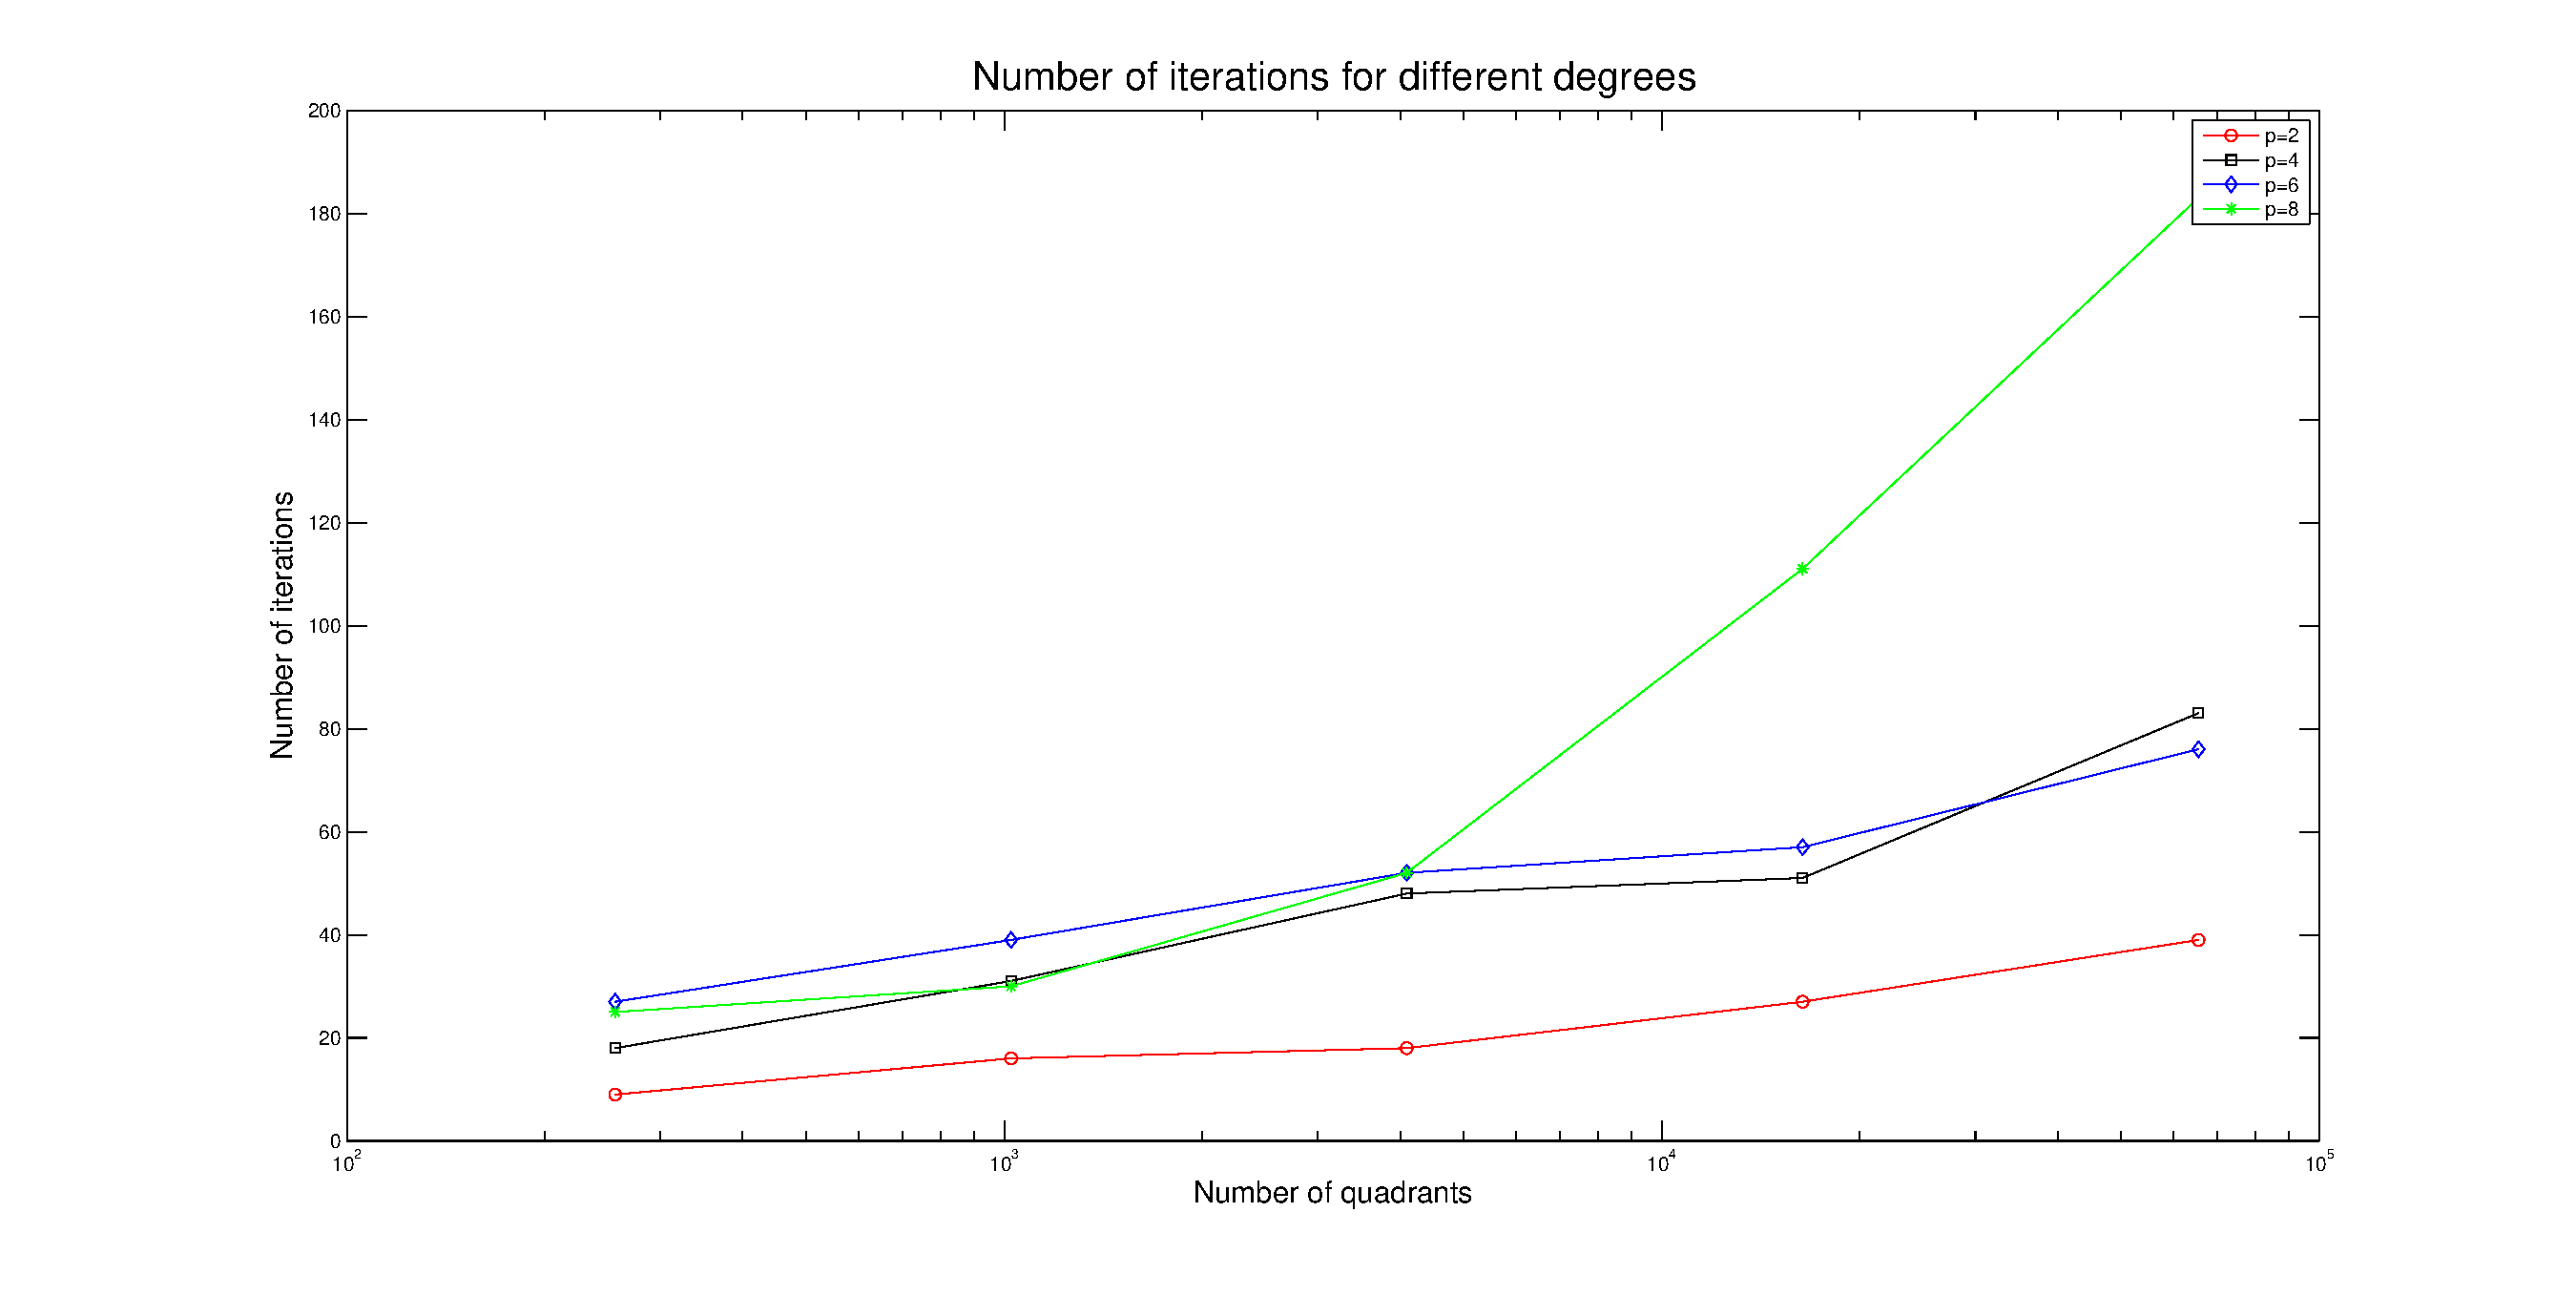
\includegraphics[scale=0.35]{Results/fine_reg_iter.eps}
\caption{Number of iterations of PCG with only the fine preconditioner for different degree $p$ of interpolation as a function of the number of quadrants in a regular mesh.}
\label{fine_reg_iter} 
\end{figure}

We can see that, even without the coarse preconditioner, we are solving the system in a small number of iterations compared to the number of degrees of freedom. For example, we only do about 80 iterations to solve the system with $2.4\: 10^{6}$ degrees of freedom and with interpolations of degree $p=6$. 

 We can also see that for every degree, the number of iterations increases when we refine the mesh. This is to be expected since the information from the boundaries has to go through more quadrant before propagate to the entire domain. Asymptotically, the number of iterations is expected to double as the number of quadrants is multiplied by four (i.e. the mesh size is divided by two). We can see that it is not yet the case here.

A last remark we can make is that the number of iterations tends to increase when the degree of the interpolation increases. This is especially true for the finest mesh where we need 183 iterations for $p=8$ where we only need 39 iterations for $p=2$. This can be explained by the fact that the size of the overlap decreases when $p$ grows. As mentioned in \textcolor{red}{Ref here!!}, this issue would be fixed if we imposed a constant overlap.

\subsubsection{Meshes with distorted elements}
Let us now move on to meshes that are not regular anymore. Let us remember that when we developed the fine preconditioner, we assumed that the elements were rectangular which allowed us to compute the analytic solution to the problem. This part explores the influence of having distorted elements on the number of iterations needed to obtain a given accuracy.   

\subsection{Influence of hanging nodes}




 
